\documentclass{report}
\usepackage{amsmath}
\usepackage{amssymb}
\usepackage{graphicx}
\usepackage{hyperref}
\usepackage{color}
\begin{document}
\title{Theory of Polymer Dynamics}
\maketitle
\section{Introduction}
This document summarizes information related to the construction of theoretical models representing polymers. 
It is mainly drawn from the books by Doi \cite{doi1986theory}\cite{doi1996introduction}, and Bird \cite{bird1987dynamics}. 
 
\section{The freely jointed chain}\label{section_theFreelyJointedChain}
From \cite{doi1986theory}.We start with a simple model: a chain consisting of $N$ links, each of length $b_0$ and able to point in any direction independently of each other. The conformation of the model is represented by $(N+1)$ position vectors $\{R_n\}=\{R_0,R_1,...,R_{N}\}$, or by the set of bond vectors $\{r_n\}=(r_1,r_2,...,r_N)$, where $r_n=R_{n}-R_{n-1}$. 

Since the bonds are independent, the configuration distribution is defined as 
\begin{equation*} 
\Psi(\{\vec{r}_n\})=\prod_{n=1}^N\psi(\vec{r}_n)
\end{equation*}
for vector of constant length $b_0$
\begin{equation*}
\psi(\vec{r})=\frac{1}{4\pi b_0^2}\delta(|\vec{r}|-b_0)
\end{equation*}
we then normalize such that 
\begin{equation*}
\int \psi(\vec{r})d\vec{r} =1
\end{equation*}
If the bond vectors are presented using spherical coordinates with angles $\theta$ and $\phi$, then the configuration distribution of the chain is given by 
\begin{equation*}
\psi(\theta^{N},\phi^{N})=\left(\frac{1}{4\pi}\right)^{N} \prod_{i=1}^{N}\sin(\theta_i)
\end{equation*}
This is due to the fact that the surface element of the sphere is given by the determinant of the Jacobi matrix, $J$, of spherical transformation for each $R_i=(x,y,z)$, namely
\begin{eqnarray*}
x &=& b_0\sin(\theta)\cos(\phi)\\
y &=& b_0\sin(\theta)\sin(\phi)\\
z &=& b_0\cos(\theta) 
\end{eqnarray*} 
which is $|J|=b_0^2\sin(\theta)$, to get the probability that a bond vector is in the range $d\theta d\phi$, we divide $|J|$ by the surface area of the sphere which is $4\pi b_0^2$ to get $\sin(\theta)/4\pi$ for each bond vector. Since the bond vectors are independent, we get the multiplicative expression for $\psi$.
 
Any average quantity $B(\theta,\phi)$ that depends on the configuration of the chain in equilibrium will be written as  
\begin{equation*}
\left< B\right>=\int\int B \psi d\theta^{N}d\phi^{N}
\end{equation*}
The above property of expected value of a quantity $g(x)$ given that we know only the distribution function $f(x)$ is the called the \textbf{Law of the unconscious statistician}.
\begin{equation*}
E[g(x)]=\int_{-\infty}^{\infty}g(x)f(x)dx = \int_{-\infty}^{\infty}g(x)dF(x)dx
\end{equation*} 
were $F(x)$ is the cdf (if known).

\subsection{The end-to-end vector}\label{subsection_theEndToEndVector}
We define the end-to-end vector as $\vec{R}=\vec{R}_N-\vec{R}_0=\sum_{n=1}^N \vec{r}_n$. The quantity $\left<R^2\right>$ characterizes the length of the chain. The standard deviation of the end-to-end vector
\begin{equation*}
\bar{R}=\left<R^2\right>^{0.5}=\left<(R_N-R_0)^2\right>^{0.5}=\sqrt{N}b_0
\end{equation*} 
since 
\begin{equation*}
\left<R^2\right> = \left<\left(\sum_{n=1}^N(r_n)\right)^2\right>=\sum_{n=1}^N\sum_{m=1}^N\left<r_nr_m\right>+\sum_{n=1}^N\left<r_n^2\right>+2\sum_{m>n}^N\left< r_nr_m\right>=\sum_{n=1}^N\left<r_n^2\right>=Nb_0^2
\end{equation*}

therefore, $\left<R^2\right>^{0.5}=\sqrt{N}b_0$. Here we used  $\left<r_nr_m\right>=\left<r_n\right>\left<r_m\right>=0$. Note that this is just the sum of variances of the bond vectors (each of which has variance of $b_0$)

\subsection{Distribution of the end-to-end vector}\label{subsection_distributionOfTheEndToEndVector}
We denote $\Phi(R,N)$ as the probability distribution function that the end-to-end vector of a chain of N beads is $R$.
\begin{equation*}
\Phi(R,N) =\int\int\int...\int\delta(R-\sum_{n=1}^Nr_n)\Psi(\{r_n\}))dr_1dr_2...dr_N
\end{equation*}
in short, we take all chain configurations for which the end-to-end vector is exactly $R$. Using the Fourier transform identity for the delta function
\begin{equation*}
\delta(r)= \frac{1}{(2\pi)^3}\int e^{ikr} dk
\end{equation*}
see \href{http://en.wikipedia.org/wiki/Dirac_delta_function}{wikipedia}.
where, after some manipulation and using polar coordinates for solving the integral, we get
\begin{equation*}
\Phi(R,N)=\frac{1}{(2\pi)^3}\int e^{ikR} \left(\frac{\sin(kb)}{kb}\right)^N dk
\end{equation*}
Continuing with a series of approximations to the integral above, we get
\begin{equation*}
\Phi(R,N)=(3/2\pi N b^2)^{1.5} \exp(-\frac{3R^2}{2Nb^2})
\end{equation*}


\section{The Gaussian Chain}\label{section_theGaussianChain}
From \cite{doi1986theory}. We consider a chain whose bond length has a Gaussian distribution 
\begin{equation*}
\psi(r)=\left[\frac{3}{2\pi b^2} \right]^{3/2} \exp \left( -\frac{3r^2}{2b^2} \right)
\end{equation*}
in 3D,  with bond-length variance $<r^2> =b^2$. The Gaussian chain represent the model of beads on a strings, with the harmonic potential energy 
\begin{equation*}
U_0(\{R_n\})\frac{3k_BT}{2b^2}\sum_{n=1}^N (R_n-R_{n-1})^2
\end{equation*}

Since the sum of two Gaussian random variables is again a random variable, it turns out that the distribution of the bond between any two beads $m$ and $n$ is Gaussian with 
\begin{equation*}
\Phi(R_n-R_m,n-m)=\left[\frac{3}{2\pi b^2 |n-m|}\right]^{3/2}\exp \left[-\frac{3(R_n-R_m)^2}{2|n-m|b^2}\right]
\end{equation*}
and for any $m$ and $n$ 
\begin{equation*}
<(R_n-R_m)^2> = |n-m|b^2
\end{equation*}

From the formula of the distribution, we can immediately see that setting $R_N=R_m$, meaning placing two beads at the same position, gives us the encounter probability at steady state, namely $A|n-m|^(3/2)$, with $A$ some constant of normalization. 

We can thus immediately see that when setting $R_n=R_m$ we get 
\begin{equation*}
\Phi(0,|n-m|)=(3/2\pi b^2 |n-m|)^{1.5}
\end{equation*}
which is the steady state probability of encounter, which drops with the distance





\section{The Rouse Chain}\label{section_theRouseChain}
From \cite{doi1986theory} Chap. 4. The Rouse model was suggested as the basis for polymer dynamics in dilute solution. Let $\{R\}=\{R_1,R_2,...,R_N\}$ be the coordinates of the beads of the chain. The motion of the beads is described using the Smoluchowski equation
\begin{equation*}
\frac{\partial \Psi}{\partial t }=\sum_n \frac{\partial}{\partial R_n}H_{nm}\left[k_BT\frac{\partial \Psi}{\partial R_m}+\frac{\partial U}{\partial R_m}\Psi\}\right]
\end{equation*}

\subsection{The source of the Hookian behavior}\label{subsection_sourceOfTheHookianBehavior}
From \cite{bird1987dynamics}. Let us look at the probability density function of the end-to-end vector being length $r$ at equilibrium
\begin{equation*}
P_{eq}(r)= \left(\frac{3}{2\pi (N-1)b^2}\right)\exp(-3r^2/2(N-1)b^2)
\end{equation*}

 The Helmholtz free energy $A=U-TS$, with $U$ the internal energy and $S$ the entropy, of the system in equilibrium at temperature $T$ is given by 
\begin{equation*}
A=-KT\ln(Z)
\end{equation*}
with $Z$ the partition function, which is defined as 
\begin{equation*}
Z=c\int e^{(\mathbb{K+\phi})/(KT)}
\end{equation*}
with $c$ some constant,$\mathbb{K}$ is the kinetic energy of the system, $\mathbb{\phi}$ is the potential energy, over the phase space of the system. 

When the length of the chain is changed by a small amount, the change in the Helmholtz free energy is 
\begin{equation*}
dA=-KTd\ln{P_{eq}}=\frac{3KT}{(N-1)b^2}(r\cdot dr)
\end{equation*}

We also know that the change in the Helmholtz free energy is related to the tension $F^c$ of the chain by 
\begin{equation*}
dA=(F^c\cdot dr)
\end{equation*}
equating these two quantities we get 
\begin{equation*}
F^c(r) = -\frac{3KT}{(N-1)b^2}r	 \qquad N-large
\end{equation*}
therefore, we see that the tension behaves as a Hookian spring. If we set $N=2$ we get the spring constant between any two beads.

We can therefore write the probability density function for the end to end vector using the Hookian spring constant
\begin{equation*}
P(r)= \left(\frac{k}{2\pi KT}\right)^{1.5}\exp\left(-\frac{k r^2}{2KT}\right)
\end{equation*}

\subsection{The center of mass}\label{subsection_theCenterOfMass}

The center of mass is defined as the mean bead position over time 

\begin{equation*}
cm(t) = \frac{1}{N+1}\sum_{i=0}^N{R_n(t)}
\end{equation*}

therefore, the differential equation for the center of mass is 

\begin{equation*}
\frac{dcm}{dt}=\frac{1}{N+1}\sum_{i=0}^N{\frac{dR_i}{dt}}= \frac{1}{N+1}\sum_{i=0}^Nf_n(t)
\end{equation*}

\subsection{Central bead is closest to the center-of-mass}\label{subsection_centralbeadClosestToCenterOfMass}
In this subsection we show that on average the central beads of the chain are closest to the center of mass of the chain. This result will be useful in future sections when we calculate the encounter probability between beads in the chain with beads outside of it, to be the multiplication of the probability of an encounter between a bead outside the loop with a phantom bead in the center of mass of the loop and the encounter between beads in the loop and its center of mass. 

Let our chain be defined as a sequence of $N$ uncorrelated and independent random variables in the following way\\
$p_1 = n_1$\\
$p_2 = p_1+n_2=n_1+n_2$\\
$p_3 = p_2+n_3=n1+n_2+n_3$\\
.\\
.\\
$p_N = \sum_{i=1}^{i=N}n_i$\\
where $n_i\sim N(0,1)\forall i=1..N$ and $N$ is an odd integer.

We define the chain center of mass as:
\begin{equation*}
p_{cm}=\frac{1}{N}\sum_{i=1}^{i=N}p_i = \frac{1}{N}(Nn_1+(N-1)n_2+(N-3)n_3+...n_N)=\sum_{i=1}^{N}(\frac{N-i+1}{N})n_i
\end{equation*}

The question we address here is for which index $k\in[1..N]$ does the point $p_k$ is closest to $p_{cm}$?

Each $p_i$ is distributed normally with mean $\mu_i =0$ (since the sum of means of the preceding points is zero) and $\sigma_i=\sqrt{\sigma_{i-1}^2+1+2\rho\sigma_{i-1}}$, where $\rho$ is the correlation coefficient. Since each two subsequent points are uncorrelated, by definition $\rho=0$. More specifically, the $\rho$ in the expression for the standard deviation of point $i$ is given by $E[(n_i-\mu_i)(p_{i-1}-\mu_{i-1})]/\sigma_{n_i}\sigma_{i-1}=E[n_ip_{i-1}]/\sigma_j$, where $E$ is the expectation. Since $n_i$ is independent of $p_{i-1}$, we get
\begin{equation*}
E[n_ip_{i-1}])=E[n_i]E[p_{i-1}]=0
\end{equation*}
Therefore we get 
\begin{equation*}
\sigma_i=\sqrt{i}
\end{equation*}

The center of mass $p_{cm}$ has mean $\mu_{cm}=0$ and standard deviation that can be written as
\begin{equation*}
\sigma_{cm}=\sum_{i=1}^{i=N}\left( \frac{N-i+1}{N}) \right)^2 = \frac{N(N+1)(2N+1)}{6N^2}
\end{equation*}

We now look for the point $p_j$ for which the distribution of the random variable 
\begin{equation*}
Y(j)=p_{cm}-p_j
\end{equation*}
is the most 'concentrated' around zero. 
In this sense, the standard deviation of $Y(j)$ should be the smallest among all $i=1..N$.

the random variable $Y(j)$ can be written as
\begin{equation*}
Y(j) = \sum_{k=1}^{N}\left(1+\frac{1-k}{N}\right)n_k -\sum_{k=1}^{j}n_k = \sum_{k=1}^{j}\frac{1-k}{N}n_k +\sum_{k=j+1}^{N}(1+\frac{1-k}{N})n_k
\end{equation*}

The standard deviation of $Y_j$ is
\begin{equation*}
\sigma_{Y(j)}=\sqrt{\sum_{k=1}^{j}\left(\frac{1-k}{N}\right)^2+\sum_{k=j+1}^{N}\left(\frac{N+1-k}{N} \right)^2}=\frac{1}{N}\sqrt{\sum_{k=1}^{j-1}k^2+\sum_{k=1}^{N-j}k^2}
\end{equation*}
To find the $j$ that minimizes this expression, we can disregard the square root, and denote $Q(j)=\sum_{k=1}^{j-1}k^2$, so $Q(N-j+1)=\sum_{k=1}^{N-j}k^2$. Differentiate to find $Q'(j)-Q'(N-j+1)=0$  we see that when $j= \frac{N+1}{2}$\\
\begin{equation*}
Q'(\frac{N+1}{2})-Q'(N-\frac{N+1}{2}+1)=Q'(\frac{N+1}{2})
\end{equation*} 




\subsection{The distribution of the bond lengths}\label{subsection_distributionOfTheBondLength}
[UNFINISHED] 

The bond length behaves like the central $\chi ^2$ with $d$ degrees of freedom, where $d$ is the dimension of the problem. 
In $3D$, since each $\vec{r}_i=[x_i,y_i,z_i]$ has 3 coordinates, each i.i.d normally distributed with $\left<x_i^2\right>=\left<y_i^2\right>=\left<z_i^2\right>=\frac{b^2}{3}$, the length squared $\|\vec{r}_i\|^2=x_i^2+y_i^2+z_i^2\sim\chi^2(3)$ 
with variance $\mu=b^2/3+b^2/3+b^2/3=b^2$ which is the sum of variances.

To calculate the cumulative distribution function (CDF) of the bond length, we use result from the analysis of quadratic forms \cite{mathai1992quadratic} (chapter 3). From the CDF we will obtain the \textit{survival probability}, which its first moment is the \textit{mean first passage time} for the two ends of the polymer.

For the polymer chain, the bond length is a random variable, $b\sim \mathcal{N}(0,\sigma_b)$
\subsection{Eigenvalues of the Rouse Matrix}\label{subsection_eigenvaluesOfTheRouseMatrix}
In this subsection we derive the eigenvalues of the Rouse matrix. The Rouse matrix defines the connection between beads as a harmonic potential. The system of differential equation governing the dynamics of the chain comprised of $N$ beads is 
\begin{equation}
\frac{d[X(t)]}{dt}=-k[R][X(t)]+[g(t)]
\end{equation}
where the $[.]$ notation represents a matrix (vector), $[g(t)]$ is an $N$ by 1 vector of normally distributed numbers with mean 0 and STD =1, $k$ is a constant and the matrix $[R]$ is defined as:
\begin{equation}
R=\left[
\begin{matrix}
 1 & -1 &  0 &  0 &...&  &  0 \\
-1 &  2 & -1 &  0 &...&  &  0 \\
 0 & -1 &  2 & -1 &...&  &  0 \\
 . &    &    &  . &   &  &  . \\
 . &    &    &  . &   &  &  . \\
 0 &    &    &    & -1& 2& -1 \\
 0 &    &    &    &  0&-1&  1 \\     
\end{matrix}
\right]
\end{equation}
The Rouse matrix is also called the Kirchhoff matrix of the chain's graph.

To find the eigenvalues we calculate 
\begin{equation*}
D_N=\left|[R]-\lambda[I]\right|=0
\end{equation*}
which gives us a matrix of the form 
\begin{equation*}
R=\left[
\begin{matrix}
 y & -1 &  0 &  0 &...&  &  0 \\
-1 &  x & -1 &  0 &...&  &  0 \\
 0 & -1 &  x & -1 &...&  &  0 \\
 . &    &    &  . &   &  &  . \\
 . &    &    &  . &   &  &  . \\
 0 &    &    &    & -1& x& -1 \\
 0 &    &    &    &  0&-1&  y \\     
\end{matrix}
\right]
\end{equation*}
with $x=2-\lambda$, and $y=x-1$.

Developing the determinant by the last column we find a recursion relation as follows 
\begin{equation*}
D_N = yD_{N-1}-D_{N-2}
\end{equation*}

Since the recursion relation is slightly different for $D_{N-1}$, bt remains the same for all $j\leq N-1$, we solve the recursion relation for $D_{N-1}$ and then return to define the last term $D_N$ using the relation above. 

The recurrence relation is:
\begin{equation*}
D_z = xD_{z-1}-D_{z-2}
\end{equation*}

with the boundary conditions
\begin{equation*}
D_1 = y 
\end{equation*}
\begin{equation*}
D_2 = xy-1
\end{equation*}
We note that according to the Rouse matrix $x=y+1$.

The particular solution to the recursion relation is 
\begin{equation*}
D_z=e^{iz\theta}
\end{equation*}

substituting it into the recursion relation gives
\begin{equation*}
e^{iz\theta}=xe^{i(z-1)\theta}-e^{i(z-2)\theta}
\end{equation*}

hence
\begin{equation*}
x=2cos(\theta)
\end{equation*}

The general solution can then be defined as 
\begin{equation*}
D_z=Ae^{iz\theta}+Be^{-iz\theta}
\end{equation*}
where $A$ and $B$ are some constants to be defined.

 Using the boundary conditions we get 
 \begin{equation*}
 y = Ae^{i\theta}+Be^{-i\theta}
 \end{equation*}
 
 \begin{eqnarray*}
 A & = & \frac{y-Be^{-i\theta}}{e^{i\theta}} = (2\cos(\theta)-1)e^{-i\theta}-Be^{-2i\theta}\\
   & = & \frac{1-e^{i\theta}}{e^{-i\theta}-e^{i\theta}} = e^{i\theta/2}\frac{e^{-i\theta/2}-e^{i\theta/2}}{-2i\sin(\theta)}\\
   & = & \frac{e^{i\theta/2}}{2\cos(\theta/2)}
 \end{eqnarray*}
 and 
 \begin{equation*}
 B=\frac{e^{-i\theta}-1}{e^{-i\theta}-e^{i\theta}}=\frac{e^{-i\theta/2}}{2cos(\theta/2)}
 \end{equation*}
The general solution is now
\begin{equation}
D_z=\frac{e^{i\theta/2}}{2\cos(\theta/2)}e^{iz\theta}+\frac{e^{-i\theta/2}}{2\cos(\theta/2)}e^{-iz\theta}=\frac{\cos((z+1/2)\theta)}{\cos(\theta/2)}
\end{equation}
Since the determinant must vanish, we have 
\begin{equation*}
D_N = yD_{N-1}-D_{N-2}=0
\end{equation*}
substituting the expressions for $D_{N-1}$ and $D_{N-2}$ into the equation above yields 
\begin{equation*}
yD_{N-1}-D_{N-2} = D_1D_{N-1}-D_{N-2} = 
\end{equation*}
\begin{equation*}
\frac{\cos(3\theta/2)}{\cos(\theta/2)}\frac{\cos((N-1/2)\theta)}{\cos(\theta/2)}-\frac{\cos((N-3/2)\theta)}{\cos(\theta/2)}=0
\end{equation*}
therefore 
\begin{equation*}
\cos(3\theta/2)\cos((N-1/2)\theta)=\cos((N-3/2)\theta)\cos(\theta/2)
\end{equation*}
displaying the trigonometric functions as sum of exponentials we can get
\begin{equation*}
\cos((N+1)\theta)-\cos((N-1)\theta)=0
\end{equation*}
which gives 
\begin{equation*}
-2\sin(N\theta)\sin(\theta)=0
\end{equation*}
therefore 
\begin{equation*}
\theta = \frac{p\pi}{N}
\end{equation*}
$p=0,1...,N-1$ (since we have $N$ solutions)\\

The eigenvalues are then
\begin{equation*}
\lambda_p=2-x = 2-2\cos(\theta_p)=2\left(1-\cos(\frac{p\pi}{N})\right)=4\sin^2(\frac{p\pi}{2N})
\end{equation*}
$p=0,1,...,(N-1)$.

\subsection{Eigenvectors of the Rouse Matrix}\label{subsection_eigenvectorsOfTheRouseMatrix}
[Show Full derivation]

The $k^{th}$ entry in the $p^{th}$ eigenvector is 

\begin{equation*}
c_k = \sqrt{\frac{2}{N}}\sin(\frac{k\pi p}{N})
\end{equation*}

with $k=1,2,..,N$ and $p=0,1,...N-1$

\subsection{Centralizing the chain}\label{subsection_centralizingTheChain}
[UNFINISHED]

The differential equation describing the dynamics $R_n$ in $3D$ is

\begin{equation*}
\frac{dR_n}{dt} = -\frac{3D}{b^2}\left(2R_n(t)-R_{n-1}(t)-R_{n+1}(t) \right)+f_n(t)
\end{equation*}

If we shift the chain so that its new center of mass always lays at the origin, we get 

 \begin{equation*}
\frac{d(R_n-cm)}{dt} = -\frac{3D}{b^2}\left(2R_n-R_{n-1}-R_{n+1} \right)+f_n-\frac{1}{N+1}\sum_{i=0}^Nf_i
\end{equation*}

for such a new system, the new center of mass, $cm^*$ should have zero derivative, indeed. 
\begin{equation*}
\frac{dcm^*}{dt}=\frac{1}{N+1}\left[ \sum_{i=1}^N\frac{dR_i}{dt} - (N+1)\sum_{i=0}^N\frac{1}{N+1}f_i \right]= \vec{0}
\end{equation*}
Of course, this process is only valid post simulation. It seems not plausible to simulate a random process such that its center of mass remains in one point. 

Subtracting the center of mass from the position of each bead should not affect the distribution of bond lengths, and it is indeed obvious to see it by subtracting two consecutive beads equation that the center of mass cancels out. However, the distribution of bead position is affected. 

since each $f_n$ is normally distributed with std $\sqrt{2D}$ and mean 0, the random variable $\frac{1}{N}\sum_{i\neq n}^Nf_n(t)$ 


\subsection{Mean First End To end Encounter Time Of the Rouse Chain}\label{subsection_meanEndToEndEncounterTimeOfTheRouseChain}
From \cite{amitai2012computation}. [UNFINISHED]

\subsection{The Pair Correlation function}\label{subsection_thePairCorrelationFunction}
According to \cite{doi1996introduction}. To investigate the spatial distribution of segments in the Rouse polymer we introduce the segment pair correlation function, $g(r)$, defined as follows. If we focus on the $n^{th}$ segment, we define $g_n(r)$ to be the average segment density at position $r$ from segment $n$. If we write $R_n(n=1,2,3,..,N)$ for the position vectors of the segments , then we can express $g_n(r)$ as 
\begin{equation*}
g_n(r)=\sum_{m=1}^N \left<\delta(r-(R_m-R_n)) \right>
\end{equation*} 

The average is a spatial average, so in 3D we have to divide by the volume $r+\delta r$ to get the concentration. The time correlation function, $g(r)$, is then defined as the average of the segment pair correlation function, $g_n(r)$. 
\begin{equation*}
g(r) = \frac{1}{N}\sum_{n=1}^{N}g_n(r)
\end{equation*}
In addition, we define $g(q)$, the Fourier transform of $g(r)$
\begin{equation*}
g(q) = \int e^{iqr}g(r)dr = \frac{1}{N}\sum\limits_{n=1}^{N}\sum\limits_{m=1}^{N}\left<exp([iq(R_m-R_n]) \right>
\end{equation*}
The pair correlation function is thus also called the radial distribution function. In the simplest terms it is a measure of probability of finding a particle at a distance $r$ away from a given reference particle. 


\subsection{Radius of Gyration}\label{subsection_radiusOfGyration}
[UNFINISHED]

From the definition of the Fourier transform of the pair correlation function for small $q$, we can define the length called radius of gyration. 

\section{The Rouse ring}\label{section_theRouseRing}
Construction of the Rouse ring is done by setting the first and last beads at position $x_0=0$. This forms a discrete \textbf{Brownian bridge}, which is defined using the standard random walk, $w(t)$, with $\left<w(t)^2\right>=1, \left<w(t)\right>=0$, of $N$ steps (between $N+1$ beads). 
\begin{equation*}
B(t)= w(t)-\frac{t}{N}w(N) \qquad t=1,..,N
\end{equation*} 

In the context of polymer dynamics we will refer to the bridge as a \textit{Rouse ring}. The expectation $E[B(t)]$ can be shown to be 0 due to the properties of the Brownian paths
\begin{equation*}
E[B(t)]=E[w(t)-\frac{t}{N}w(N)]=E[w(t)] -(t/N)E[w(N)]=0
\end{equation*}

The covariance, $C_B$, of $B(t)$ is 
\begin{eqnarray*}
C_{B}  & = & E((B(t)-E[B(t)])(B(s)-E[B(s)])\\
   & = & E[B(t)B(s)]=E[(w(t)-(t/N)w(N))(w(s)-(s/N)w(N))]\\
   & = & E[w(s)w(t)-w(N)(sw(t)+tw(s))/N +(st/N^2)w(N)^2 ]\\
   & = & min(s,t)-(s/N)min(N,t)-(t/N)min(N,s)+st/N^2\\
   & = & min(s,t)-2st/N+st/N^2\\
   & = & min(s,t)-(st/N^2)(2N-1)
\end{eqnarray*}

We therefore see that the position of the Rouse ring are dependent. The variance is given by setting $s=t$ to be 
\begin{equation*}  
\sigma^2_{B}=t-(t/N)^2(2N-1)
\end{equation*}

The Rouse ring is a Gaussian process with a joint probability density function  given by  
\begin{equation*}
f_B(x)=\frac{1}{\sqrt{((2\pi)^N|C_B|)}}\exp(-0.5x^TC_B^{-1}x)
\end{equation*}

\subsubsection{Derivation of the probability density of the Rouse ring}
The Rouse ring is a tied-down random walk, with $w(N)=w(0)$. Without loss of generality, we set $w(0)=0$, as in the classical random walk.

The probability density function of the random walk in 3D is given by the Weiner measure as  
\begin{equation*}
f(w(x),N)=\left( \frac{1}{2\pi N}\right)^{3/2}\exp(-\frac{3x^2}{2N^2})
\end{equation*}

Conditioning the random walk on the event that $w(N)=w(0)$ we get 
\begin{eqnarray*}
f(0,x,0;0,t/N,N)&=&\frac{1}{\sqrt{(2\pi)^2 t(N-t/N)/N}}\exp(-\frac{x^2}{2t/N}-\frac{x^2}{2(N-t/N)})\\
&=&\frac{N}{2\pi\sqrt{t(N-t)}} \exp(-\frac{x^2}{2t(N-t)/N^2})
\end{eqnarray*}
and in 3D
\begin{equation*}
f(0,x,0;0,\frac{t}{N},N) = \left(\frac{N}{\sqrt{2\pi t(N-t)}}\right)^3 \exp\left(-\frac{xx^T}{2t(N-t)/N^2}\right)
\end{equation*}

\subsection{Encounter probability in the Rouse ring}\label{subsection_encounterProbabilityInTheRing}
The vector between bead 1 and bead $m$ of the chain has the probability density 
$f(0,x,0;0,\frac{m}{N},0)$. Since in the ring we cannot distinguish between beads, we see that the encounter probability at equilibrium between beads $m$ and $n$ is 
$f(0,0,0;0,\frac{|m-n|}{N},0)=\left(\frac{N}{2\pi \sqrt{|m-n|(N-|m-n|)}}\right)^3$

To normalized the quantity above we write 
\begin{equation*}
f(0,x,0;0,\frac{m}{N},0)=\left(\frac{N}{2\pi\sqrt{m(N-m)}}\right)^3 /\sum_{t=1}^{N-1}\left(\frac{N}{2\pi\sqrt{t(N-t)}}\right)^3 
\end{equation*}
which is the encounter probability at equilibrium between two beads with a distance $m$ along the ring between them (note the symmetry between $m$ and $N-m$). 

\begin{figure}[h!]
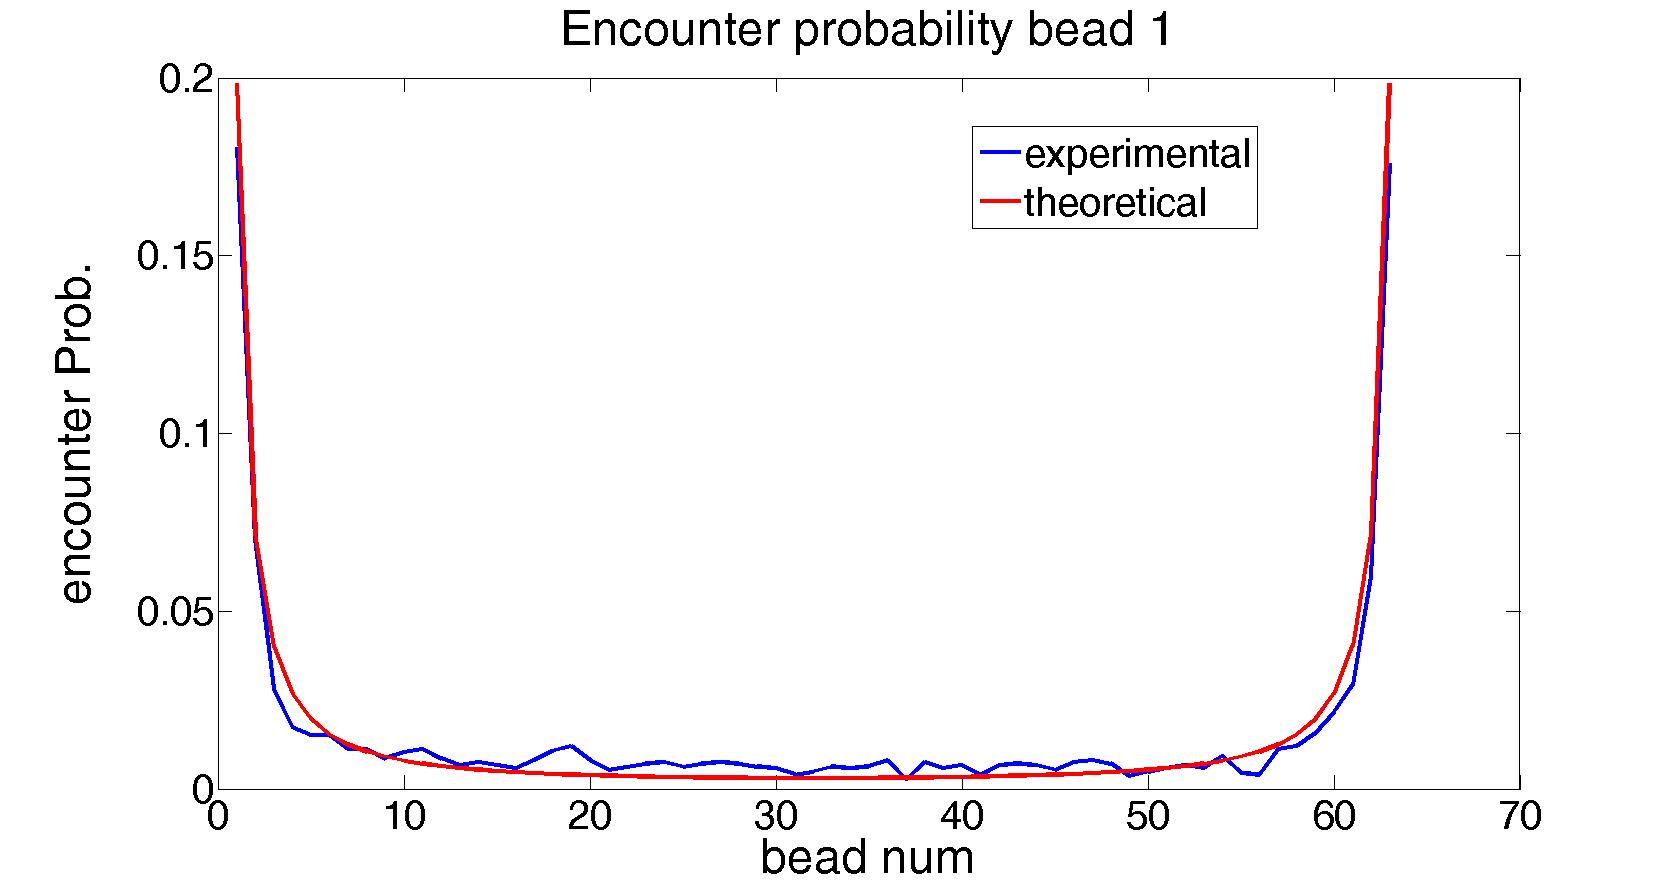
\includegraphics[scale=0.2]{encounterProbBead1InLoopOf64BeadsSimpleRouse}\caption{Encounter Probability of bead 1 in a ring of 64 beads (blue) from 10,000 simulation compared to the theoretical result (red)}\label{figure_rouseRingEncounterProbabilityComparisionToTheory}
\end{figure}
The normalization is made in accordance to the encounter data, in which we divide all encounter frequency by the total number of encounter for each bead, to give an area under the curve of 1. 

\subsection{Configuration distribution of the Rouse ring}\label{subsection_configurationDistributionRouseRing}

The increments of the Rouse ring are
\begin{equation*}
\Delta B_t= B(t+1)-B(t)=w(t+1)-w(t)-(1/N)w(N)
\end{equation*}
which is a Gaussian process as the subtraction of two Gaussian processes, with the following properties
\begin{equation*}
E[\Delta B_t]=E[w(t+1)-w(t)-(1/N)w(T)]=0
\end{equation*}
and covariance
 \begin{eqnarray*}
 C_{\Delta} & = & E[\Delta B_t \Delta B_s]\\
  & = & min(s+1,t+1)-min(t+1,s)-min(t,s+1)\\
  &+ & min(s,t)-(1/N^2)(2N-1)
 \end{eqnarray*}
Setting $s=t $ we get the variance 
\begin{equation*}
\sigma^2_{\Delta}=1-(1/N^2)(2N-1)=\frac{(N-1)^2}{N^2}
\end{equation*}

The joint pdf of the increments is therefore 
\begin{equation*}
f_\Delta(\vec{x}) = \left(\frac{1}{\sqrt{(2\pi)^N |C_\Delta|}}\right)\exp(-0.5x^TC_\Delta^{-1}x)
\end{equation*}

To fully express $f_\Delta(x)$ we need to estimate $|C_\Delta|$ and $C^{-1}$. The form of $C_\Delta$ is 

\begin{equation*}
C_\Delta = \left[
\begin{matrix}
\sigma^2_{\Delta}     & \sigma^2_{\Delta}-1 & \sigma^2_{\Delta}-1 & ...                 & \sigma^2_{\Delta}-1 \\
\sigma^2_{\Delta}-1   &\sigma^2_{\Delta}    & \sigma^2_{\Delta}-1 & ...                 & \sigma^2_{\Delta}-1 \\
\sigma^2_{\Delta}-1   & \sigma^2_{\Delta}-1 & \sigma^2_{\Delta}   & ...                 & \sigma^2_{\Delta}-1 \\
.                     &    .                &                     &                     &      \\
.                     &                     &  .                  &                     &      \\
.                     &                     & \sigma^2_{\Delta}-1 & \sigma^2_{\Delta}   & \sigma^2_{\Delta}-1  \\
\sigma^2_{\Delta}-1   & ...                 &...                  & \sigma^2_{\Delta}-1 & \sigma^2_{\Delta}
\end{matrix}
\right]
\end{equation*}
or shortly 
\begin{equation*}
C_\Delta(s,t)=
\begin{cases}
\sigma^2_\Delta & s=t\\
\sigma^2_\Delta-1 & s\neq t\\
\end{cases}
\end{equation*}
The resulting $C_\Delta$ is a circulant matrix with normalized eigenvectors
\begin{equation*}
\omega_j = (1/\sqrt{N})(1,\omega_j,\omega_j^2,...,\omega_j^{N-1})
\end{equation*}
with $\omega_j = \exp(\frac{2\pi ij}{N}) \quad i=\sqrt{-1}$, $j=0,..,N-1$. And eigenvalues
\begin{equation*}
\lambda_j = c_0 +c_1\omega_j +c_2\omega_j^2 +..c_{N-1}\omega_j^{N-1} \quad j=0,..,N-1
\end{equation*}
where, $c_j$ is the first row of $C_\Delta$, i.e $c_0=\sigma^2_{\Delta} , c_{N-1}=..c_1=\sigma^2_{\Delta} -1$. Therefore, the eigenvalues can be written as 
\begin{equation*}
\lambda_0 =  \sigma^2_{\Delta}+(N-1)( \sigma^2_{\Delta}-1)=\frac{1-N}{N}
\end{equation*}

\begin{eqnarray*}
\lambda_j & = & \sigma^2_{\Delta} +(\sigma^2_{\Delta}-1)\sum_{n=1}^{N-1}\exp(\frac{2\pi nij}{N})\\
& = & \sigma^2_{\Delta} +(\sigma^2_{\Delta}-1)\left(\sum_{n=0}^{N-1}\exp(\frac{2\pi nij}{N})-1 \right)\\
 & = &  \sigma^2_{\Delta} +(\sigma^2_{\Delta}-1)\left(\frac{1-\exp(2\pi ij)}{1-\exp(\frac{2\pi ij}{N})}-1 \right)\\
  & =&  \sigma^2_{\Delta} -(\sigma^2_{\Delta}-1) = 1 \\
  && \quad j=1,..,N-1
\end{eqnarray*}

Therefore, the determinant is
\begin{equation*}
|C_\Delta|=\lambda_0=\frac{1-N}{N}
\end{equation*}

Te inverse, $C_\Delta ^{-1}$, is of the form
\begin{equation*}
C_\Delta^{-1}(s,t)=
\frac{1}{1-N}+\frac{1}{N}\sum_{n=1}^{N-1}(\omega_{s-1}\omega_{t-1})^n
\end{equation*}
$s=1,..,N, t=1,..,N$. Therefore,
\begin{equation*}
C^{-1}_\Delta(s,t) = 
\begin{cases}
\frac{N-(N-1)^2}{N(1-N)} & s=t\\
\frac{2N-1}{N(1-N)}      & s\neq t
\end{cases}
\end{equation*}
note, that $\frac{N-(N-1)^2}{N(1-N)}-1 = \frac{2N-1}{N(1-N)} $, so we can write 
\begin{equation*}
C^{-1}_\Delta(s,t) = 
\begin{cases}
\alpha    & s=t\\
\alpha-1  & s\neq t
\end{cases}
\end{equation*}
\begin{equation*}
 \alpha=\frac{N-(N-1)^2}{N(1-N)}
\end{equation*}
 
The configuration distribution in 3D can be written as 
\begin{equation*}
f_\Delta(\vec{x})=\left(\frac{N}{(2\pi)^N (N-1)} \right)^{1.5}\exp(-1.5\vec{x}\cdot\delta S(\vec{x} ;\alpha))
\end{equation*}
where
\begin{equation*}
\delta S(\vec{x};\alpha)=\left[
\begin{matrix}
\alpha\sum_{n=1}^N x_n -\sum_{n\neq 1}x_n\\
\alpha\sum_{n=1}^N x_n -\sum_{n\neq 2}x_n\\
\colon\\
\alpha\sum_{n=1}^N x_n -\sum_{n\neq N}x_n\\
\end{matrix}
\right]
\end{equation*}
Note, that when $\alpha=1$ the system becomes decoupled. This happens at the limit $N\rightarrow \infty$, which makes the increments of the bridge 
\begin{equation*}
\lim_{N\rightarrow \infty} \Delta B_t=\lim_{N\rightarrow \infty} w(t+1)-w(t)-(1/N)w(N)= w(t+1)-w(t)
\end{equation*}

From $f_\Delta(\vec{x})$ we see that whenever $\displaystyle \sum_{n=1}^{N}x_n = 0$ we get $\delta S(\vec{x};\alpha)=[x_1,x_2,...,x_N]$ and we retrieve the pdf of the ring. 

The term $\vec{x}\delta S(\vec{x},\alpha)$ in the exponent of the pdf, can be written in the following form 
\begin{equation*}
\vec{x}\delta S(\vec{x};\alpha)=(\alpha-1)\left( \sum_{n=1}^N x_n\right)^2 +\sum_{n=1}^N x_n^2
\end{equation*}


\subsection{Eigenvalues of the Rouse Ring}\label{subsection_eigenvaluesOfTheRouseRing}
Connecting bead 1 and $N$ to form a ring, we now search for the eigenvalues of the new \textit{Rouse ring} matrix, $R$, harboring such a connection. For this end, we have to calculate the determinant of the matrix
\begin{equation*}
D_N=|R-\lambda I|=\left|
\begin{matrix}
 x  & -1 &  0 &  0 &...&   & -1 \\
-1  &  x & -1 &  0 &...&   &  0 \\
 0  & -1 &  x & -1 &...&   &  0 \\
 .  &    &    &  . &   &   &  . \\
  . &   .&    &    &  .&   & \\
 .  &    &    & -1 & x &-1 & 0 \\
 0  &    &    &    & -1& x & -1 \\
 -1 &   .&  . & .  &  0&-1 &  x \\     
\end{matrix}
\right|_{N\times N}
\end{equation*}

with $x=2-\lambda$. We can apply to the matrix of size $(N-1)\times (N-1)$ the same procedure as before and try to solve it recursively. The boundary conditions now read
\begin{equation*}
D_1 = x; D_2 = x^2-1
\end{equation*}
According to the solution in section \ref{subsection_eigenvaluesOfTheRouseMatrix} and in \cite{lin2011polymer}, we have 
\begin{equation*}
D_{N-1}= \frac{\sin(N\theta)}{\sin(\theta)}
\end{equation*}

The relationship between $D_N$ and $D_{N-1}$ is found by developing the determinant of $D_N$ according to the last column
\begin{equation*}
D_N = x(-1)^{2N}D_{N-1}+(-1)(-1)^{2N-1}D^*+(-1)(-1)^{N+1}D^{**}=xD_{N-1}+D^*+(-1)^{N+2}D^{**}
\end{equation*}
with the determinant $D^*$ and $D^{**}$ defined as the minors 
\begin{equation*}
D^*= 
\left| \begin{matrix}
 x  & -1 &  0 &  0  &... &  0 \\
-1  &  x & -1 &  0  &... &  0 \\
 0  & -1 &  x & -1  &... &    \\
 .  &    &    &  .  &    &    \\
 .  &    &    &  .  &    &    \\
 .  &    &    &  -1 &  x &-1  \\
 -1 &    &    &     &  0 &-1  \\   
\end{matrix}\right|_{(N-1)\times(N-1)} 
D^{**}=\left|\begin{matrix}
-1  &  x & -1 &  0  &...&  0 \\
 0  & -1 &  x & -1  &...&  0 \\
 .  &    &    &  .  &   &  . \\
 .  &    &    &  .  &   &  . \\
 .  &    &    &  -1 &  x& -1 \\
 0  &    &    &     & -1& x  \\
 -1 &    &    &     &  0&-1  \\   
\end{matrix} \right|_{(N-1)\times(N-1)}
\end{equation*}
We calculate the determinants $D^*$ and $D^{**}$ by minors according to the last row to get 
\begin{equation*}
D^* = (-1)(-1)^{2N-2}D_{N-2}+(-1)(-1)^{N-1+1}(-1)^{N-2}=(-1)^{2N-1}[D_{N-2}+1]
\end{equation*}

\begin{equation*}
D^{**}=(-1)(-1)^{2N-2}(-1)^{N-2} +(-1)(-1)^{1+N-1}D_{N-2}=(-1)^{3N-3}+(-1)^{N+1}D_{N-2}
\end{equation*}
Therefore, 
\begin{eqnarray*}
D_N & = & xD_{N-1} + (-1)^{2N-1}[D_{N-2}+1]+(-1)^{N+2}[(-1)^{3N-3}+(-1)^{N+1}D_{N-2}]\\
    & = & xD_{N-1} + (-1)^{2N-1}[D_{N-2}+1]+(-1)^{4N-1}+(-1)^{2N+3}D_{N-2}\\
    & = & xD_{N-1} + D_{N-2}[(-1)^{2N-1}+(-1)^{2N+3}]+(-1)^{2N-1}+(-1)^{4N-1}\\
    & = & xD_{N-1} - 2D_{N-2}-2
\end{eqnarray*}
Substituting the solution for $D_{N-1}$ and $D_{N-2}$, we get 
\begin{equation*}
D_N = \frac{x\sin(N\theta)-2\sin((N-1)\theta)-2\sin(\theta)}{\sin(\theta)}=0
\end{equation*}

Further simplification of $D_N$ leads to 
\begin{eqnarray*}
D_N &=& 2\frac{\cos(\theta)\sin(N\theta)-[\sin((N-1)\theta)+\sin(\theta)]}{\sin(\theta)}\\
    &=& \frac{2}{\sin(\theta)}[\cos(\theta)\sin(N\theta)-[2\sin(\frac{N\theta}{2})\cos(\frac{(N-2)\theta}{2})]\\
    &=& \frac{4}{\sin(\theta)}[\cos(\theta)\sin(\frac{N\theta}{2})\cos(\frac{N\theta}{2})-\sin(\frac{N\theta}{2})[\cos(\frac{N\theta}{2})\cos(\theta)+\sin(\frac{N\theta}{2})\sin(\theta)]\\
    &=& -4\sin^2(\frac{N\theta}{2})
\end{eqnarray*}

Equating $D_N=0$ we get the solutions
\begin{equation*}
\theta_p=\frac{2\pi p}{N}
\end{equation*}
for $p=0,1,...,(N-1)$

Therefore, the eigenvalues of the Rouse ring are 
\begin{equation*}
\lambda_p=2(1-cos(\theta_p))= 2(1-cos(2\pi p/N))
\end{equation*}
Since $\cos(\frac{2\pi \phi}{N})=\cos(\frac{2\pi(N-\phi)}{N})$, we have eigenvalues multiplicities. In our case, setting $\phi=p$ we have $\cos(\frac{2\pi p}{N})=\cos(\frac{2\pi(N-p)}{N})$ for $p=1,2,3,..,(N-2)$. For the end-values, $p=0$ and $p=N-1$ the eigenvalues are unique. 

\subsection{Mean First Encounter Time in the Rouse ring}\label{subsection_meanFirstEncounterTimeInTheRouseRing}
[UNFINISHED]

Following the method in \cite{amitai2012computation}. First we transform the Rouse ring system of equation into normal coordinates using the Rouse ring eigenvalues found in Section \ref{subsection_eigenvaluesOfTheRouseRing}. We transform to normal coordinates by $u_p=\sum_{n=1}^N \alpha_p^nR_n$, where $\alpha_p$ are the eigenvectors. We then represent our boundary conditions that bead $j$ and bead $k$ are in the same position, using the normal coordinates representation. The probability density function in the normal coordinates should then satisfy the forward Fokker Planck equation. The solution to the probability density function should then be expanded as an infinite sum of the form 
\begin{equation*}
p(x,t)=\sum_{i=1}^\infty a_iw_{\lambda_i^\epsilon}(x)e^{-\lambda_i^\epsilon tD}e^{-\phi(x)}
\end{equation*}
where $w_{\lambda_i^\epsilon}(x)$ and $\lambda_i^\epsilon$ are the eigenvectors and eigenvalues of the forward Fokker Planck operator outside of the domain, and $a_i$ are coefficients. Integrate the probability density according to $x$, over the domain without the absorbing boundary (the encounter sphere), to get a function of time. An integration of the resulting function from time $t=0$ to $\infty$ is the first moment of the survival function, which is the mean first encounter time (i.e the first time the polymer's ends are at the absorbing sphere). 

\section{A ring and a chain}\label{section_aRingAndAChain}
In this section we combine the result of the Rouse chain and the Rouse ring by attaching a linear chain with a ring, reordering the indexes and deriving the encounter probability between beads in the composite structure. 

\subsection{Construction}\label{subsection_construction}
We start by attaching the a chain of $N_c-1$ beads to a ring of $N_r$ beads by connecting bead $N_c$ to an arbitrary bead in the ring. The first bead in the chain will be numbered 1. Given the choice of the connecting bead, we index the first bead in the ring as $N_c$ and the last as $N_r+N_c$. 

In equilibrium, the link vectors are independent and we can treat the two structure, the ring and the chain, separately. The first bead in the loop will be our reference point for the calculation of the encounter probability at equilibrium, by calculating the probability that both the vector $R_m-R_{N_c}$ and $R_n-R_{N_c}$ is equal to some $s$, over all possible vectors $s$.

\begin{figure}[h!]
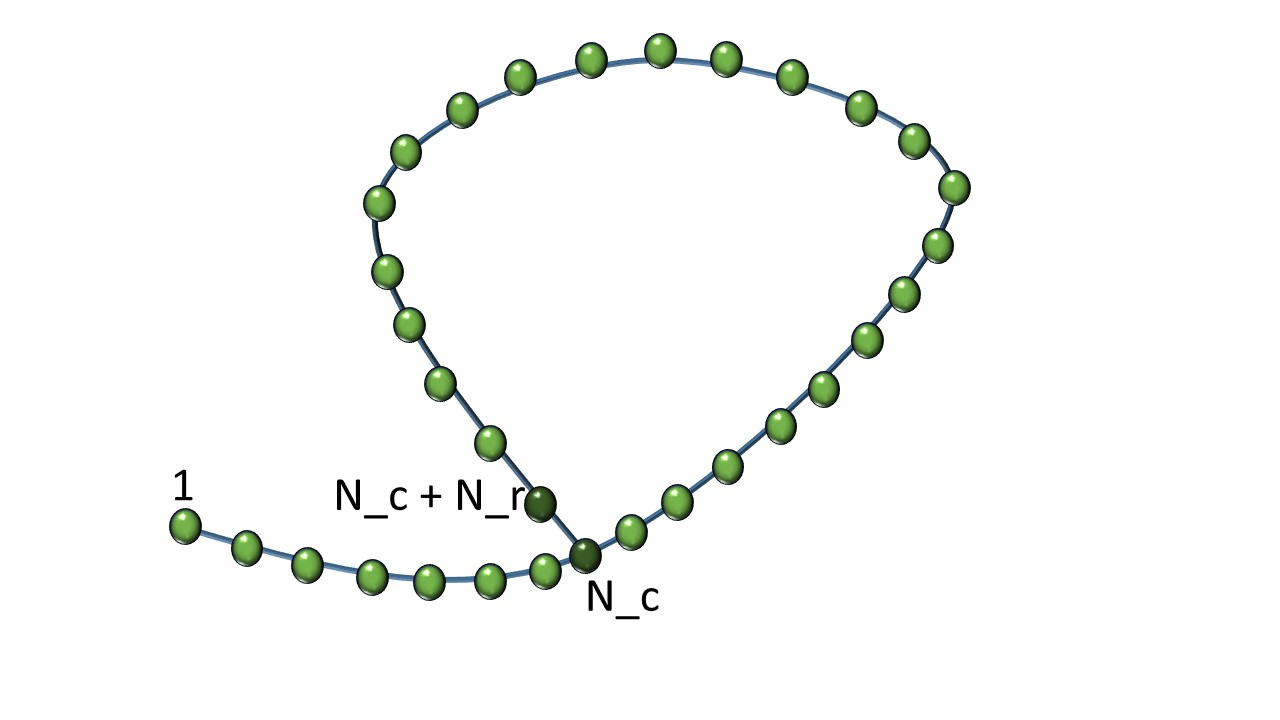
\includegraphics[scale=0.2]{chainAndRing}
\caption{A sketch of the composite structure of a chain and a ring connected}\label{figure_sketchRingChainPolymer}
\end{figure}

\subsection{The encounter probability}\label{subsection_theEncounterProbabilityChainAndRing}

We note that distribution of the vectors between bead $m$ and $n$ at equilibrium is given by 
\begin{equation*}
f_c(R_m-R_n,n-m)= \left(\frac{3}{2\pi|m-n|b^2 }\right)^{3/2}\exp(-\frac{3(R_m-R_n)^2}{2|m-n|b^2})
\end{equation*}

The Rouse ring requires a change of variables such that the steps of the Brownian bridge will be at the same scale as that of the chain. Therefore, we define our ring as the process 
\begin{equation*}
B(t)= \sqrt{\frac{N_r}{3}}b[\omega(t)-\frac{t}{N_r}\omega(N_r)]
\end{equation*}
which has the pdf 
\begin{equation*}
f_r(R_t,N_r) = \left(\frac{3}{2\pi b^2t(N_r-t)}\right)^{3/2} \exp \left(-\frac{3R_t^2}{2tb^2(N_r-t)}\right)
\end{equation*}
for the Rouse ring, with $R_t$ the vector from the connecting bead between the chain and the ring and the $t^{th}$ bead of the ring. 

Due to the independence between the structures in equilibrium, the encounter probability between bead $m$ of the chain ($1\leq m \leq N_c$) and bead $t$ ($N_c\leq t \leq N_l$) of the ring is the joint probability that $R_t-R_{N_c}= R_m-R_{N_c}=\vec{s}$. That is 
\begin{equation*}
P(R_m-R_{N_c}=\vec{s}, R_n-R_{N_c}=\vec{s})=f_r(s,N_r)f_c(s,|m-N_c|)
\end{equation*}
or, $P(R_m+R_n-2R_c=2s)$. Since the sum of these random variables is the convolution of their respective pdfs, we can perform the integration, stated in the general form for each dimension.
\begin{equation*}
f_{rc}(x)=\left(f_r*f_c\right)(x)=\left(\frac{1}{(2\pi)^2 \sigma_r\sigma_c} \right)^{1/2}\int_{-\infty}^{\infty}\exp\left(- \left(\frac{(x-y)^2}{\sigma_c}+\frac{y^2}{\sigma_r}\right)\right)dy
\end{equation*}
which can be written as
\begin{equation*}
\left(f_r*f_c\right)(x)=k\int_{-\infty}^{\infty}\exp(-fy^2+gy+h)dy
\end{equation*}
with 
\begin{eqnarray*}
k &=& \left(\frac{1}{(2\pi)^2 \sigma_c\sigma_r}\right)^{1/2}\\
f &=& \frac{\sigma_c+\sigma_r}{2\sigma_r\sigma_c}\\
g &=& \frac{x}{\sigma_c}\\
h &=& -\frac{x^2}{2\sigma_c}
\end{eqnarray*}

Using the identity for Gaussian integral, we get for 3D
\begin{equation*}
f_{rc}(x) = k\sqrt{\frac{\pi}{f}}\exp(\frac{g}{4f}+h)=\left(\frac{1}{2\pi(\sigma_c^2 +\sigma_r^2}\right)^{3/2}\exp\left(-\frac{xx^T}{2(\sigma_c^2+\sigma_r^2)}\right)
\end{equation*}
as in the classical result. with 
\begin{eqnarray*}
\sigma_c &=& (N_c-m)\frac{b^2}{3}\\
\sigma_r &=& t(N_r-t)\frac{b^2}{3}\\
\end{eqnarray*}
and $0 \leq t\leq N_r, 1\leq m\leq N_c$

The encounter probability between bead $m$ of the chain and bead $t$ of the ring is then given by 
\begin{equation*}
f_{rc}(\vec{0},m,t;N_c,N_r)=\left(\frac{3}{2\pi b^2(N_c-m+t(N_r-t))}\right)^{3/2}/S
\end{equation*}

with $S$, the normalization constant, given by 
\begin{equation*}
S= \left(\frac{3}{2\pi b^2}\right)^{3/2}\left(\sum_{n=1}^{N_c} \left(\frac{1}{n}\right)^{3/2}+\sum_{t=1}^{N_r-1} \left(\frac{N_r}{ t(N_r-t)}\right)^{3/2}\right)
\end{equation*}
$0\leq t\leq N_r$. 
We therefore see that $b$ is singled out in the calculation. 
\begin{figure}[h!]
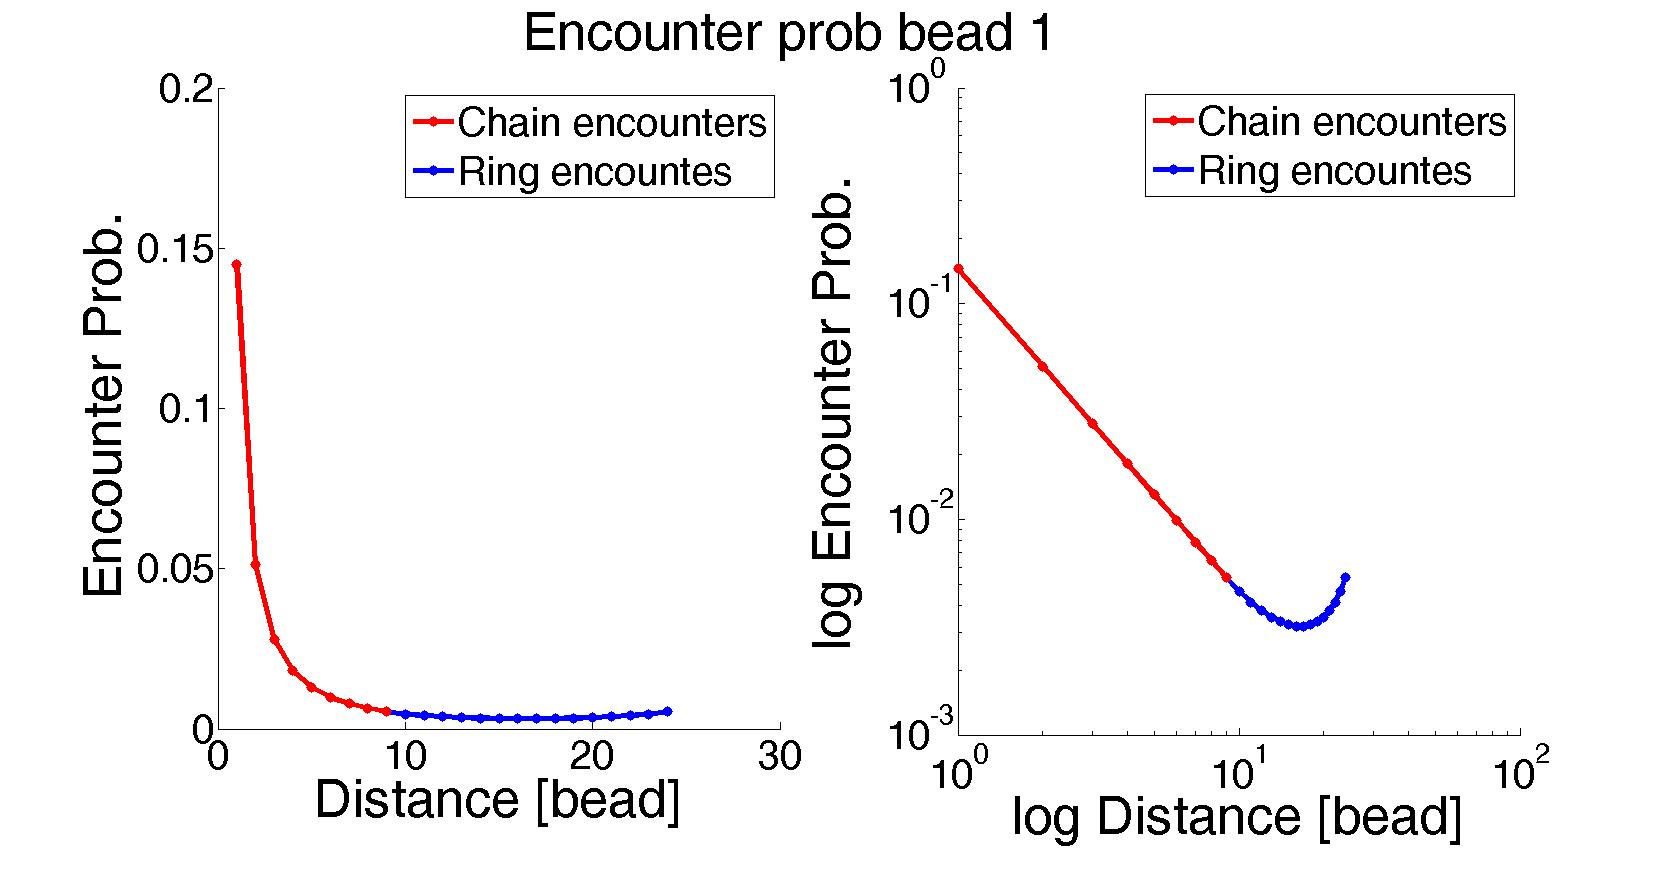
\includegraphics[scale=0.2]{encounterProbChainRingBead1}
\caption{the encounter probability of bead 1 in a bead-ring structure in linear (left) and log (right) scales. A chain of 10 beads is connected to a ring of 15 beads. The encounter probability signal is shown to be equal between beads in equal distance along the chain. For the case of the ring, the distance is the shortest distance along the graph representing the polymer} \label{figure_encounterProbChainRingBead1}
\end{figure}

\section{Two Rings}\label{section_twoRings}
We now turn to investigate the encounter probabilities between beads in a 2-ring connected structure. 
\subsection{Construction}\label{subsection_twoRingsConstruction}
We connect two Rouse rings in a signle bead, i.e there exist a bead $k$ which is shared by the two rings. The first ring is of size $N_1$, the second $N_2$
 

 
\section{Generalized Rouse Chain}\label{section_generalizedRouseChain}
Assuming a chain with $N$ beads, in which each bead is connected to its nearest neighbors and at most $N-2$ beads with spring constants $k_{ij}$ between bead $i$ and $j$. the configuration distribution of the chain is given by 
\begin{equation*}
\psi = \prod_{i=1}^{N-1}\prod_{j=1}^{N_i}\left(\frac{k_{ij}}{2\pi KT}\right)^{1.5}\exp\left(-\frac{k_{ij}r^2}{2KT}\right)
\end{equation*}
with $N_i$ the number of connections of bead $i$, with multiplication over unique pairs. 

\section{Simulations}
\subsection{Choosing $\Delta t$}
The dynamics of beads is governed by the equation
\begin{equation*}
\frac{dP}{dt} = -\frac{3D}{b^2}RP+\sqrt{2D}f_n
\end{equation*}

if we represent the Rouse matrix in its diagonal form 
\begin{equation*}
R=Q^{-1}\Lambda Q
\end{equation*}
where $Q$ is an orthonormal matrix with the eigenvectors of $R$ in its columns,and $\Lambda$ is a diagonal matrix with the Rouse eigenvalues in the diagonal, we get 
\begin{equation*}
\frac{dP}{dt} = -\frac{3D}{b^2}Q^{-1}\Lambda Q+\sqrt{2D}f
\end{equation*}
multiplying from the left by $Q$ and setting $S=QP$ we get 

\begin{equation*}
\frac{dS}{dt}=-\frac{3D}{b^2}\Lambda S+\sqrt{2D}Qf
\end{equation*}
\subsubsection{The case with no noise}
if we omit the noise term and solve for $S$ 
the numerical scheme is 
\begin{equation*}
S(t+\Delta t)-S(t)=(-\frac{3D\Delta t}{b^2}\Lambda)S(t)
\end{equation*}
taking the norm of both sides and dividing 
\begin{equation*}
\frac{\|S(t+\Delta t)-S(t)\|}{\|S(t)\|}=\|(-\frac{3D\Delta t}{b^2}\Lambda)\| = \frac{3D\Delta t}{b^2}\lambda_{max}= \frac{12D\Delta t}{b^2}
\end{equation*}
where for the Rouse matrix $\lambda_{max} = 4$.  Demanding that the quotient be smaller than 1 we have 
\begin{equation*}
 \frac{12D}{b^2}\leq1 \Longrightarrow \Delta t \leq \frac{b^2}{12D}
 \end{equation*}
 \subsubsection{The case with noise}
 using the same procedure as above, 
 \begin{equation*}
\frac{\|S(t+\Delta t)-S(t)\|}{\|S(t)\|}=\|(-\frac{3D}{b^2}\Lambda)S+\sqrt{2D}Qf\|/\|S\|\leq(\frac{3D}{b^2}\|\Lambda)\| +\sqrt{2D}\|Qf\|/\|S\|
 \end{equation*}
 \begin{equation*}
 =\leq \frac{3D}{b^2}\lambda_{max} +\sqrt{2D}\frac{\|Q\|\|f\|}{\|S\|}=\frac{12D}{b^2}\leq\frac{3D}{b^2}\lambda_{max}\Delta t +\sqrt{2D}\Delta t
 \end{equation*}
Demanding that the quotient be smaller than 1 we have 
\begin{equation*}
 \frac{12D}{b^2}\leq1 \Longrightarrow \Delta t \leq \frac{b^2}{12D+\sqrt{2D}b^2}
 \end{equation*}
\subsection{Relaxation time}
The relaxation time is determined according to the formula
\begin{equation}
\tau_p = \frac{b^2\Delta t}{12d^2\sin^2(\frac{p\pi}{2N})}
\end{equation} 

\subsection{The dynamics of bond length}\label{subsection_theDynamicsOfBondLength}
In simulations we would like to determine $\Delta t$ such that no 'blow-ups' will occur. For this end, we constrain the mean of squared difference between bond length in consecutive steps to lay below some predefined small value. 

The result show that 
\begin{equation*}
\gamma=\ll\|r_n(t+\Delta t)-r_n(t) \|^2\gg = \left(\frac{3D\Delta t}{b} \right)^2+6D\Delta t
\end{equation*}

% The bibliography
\bibliographystyle{plain}
\bibliography{TheoryOfPolymerDynamicsBibliography} % the bibliography.bib file 
\end{document}



